
\documentclass{scrartcl}
\usepackage{tikz}
\usetikzlibrary{arrows,automata}

\begin{document}
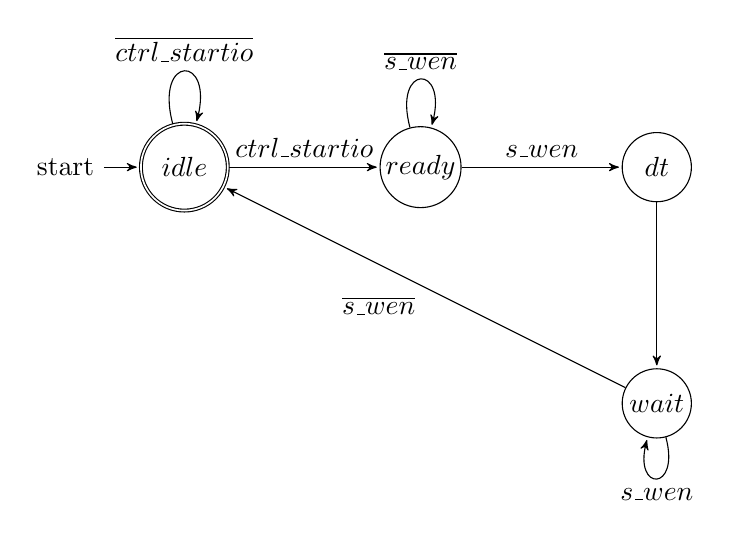
\begin{tikzpicture}[>=stealth',shorten >=1pt,auto,node distance=3cm]
  \node[initial,state,accepting, inner sep=5pt] (idle)   {$idle$};
  \node[state, inner sep=1pt]                   (ready) [right of=idle]  {$ready$};
  \node[state, inner sep=4pt]                   (dt)  [right of=ready]   {$dt$};
  \node[state, inner sep=1pt]                   (wait) [below of=dt]     {$wait$};


  \path[->]
  (idle)
  edge [loop above]
  node 
  {$\overline{ctrl\_startio}$} (idle)
  edge
  node 
  {$ctrl\_startio$} (ready)

  (ready)
  edge [loop above]
  node
  {$\overline{s\_wen}$} (ready)
  edge 
  node
  {$s\_wen$} (dt)

  (dt)
  edge 
  node
  {} (wait)

  (wait)
  edge 
  node
  {$\overline{s\_wen}$} (idle)
  edge [loop below]
  node
  {$s\_wen$} (wait)
;



\end{tikzpicture}
\end{document}
